\documentclass[dvipdfmx,autodetect-engine,titlepage]{jsarticle}
\usepackage[dvipdfm]{graphicx}
\usepackage{ascmac}
\usepackage{fancybox}
\usepackage{listings}
\usepackage{plistings}
\usepackage{itembkbx}
\usepackage{amsmath}
\usepackage{amssymb}
\usepackage{amsfonts}
\usepackage{svg}
\usepackage{url}
\usepackage{graphics}
\usepackage{listings,jvlisting}

\textheight=23cm
\renewcommand{\figurename}{図}
\renewcommand{\tablename}{表}
\newenvironment{code}
{\vspace{0.5zw}\VerbatimEnvironment  
\begin{screen} 
\baselineskip=1.0\normalbaselineskip
 \begin{Verbatim}}
{\end{Verbatim}
\baselineskip=\normalbaselineskip
 \end{screen}\vspace{0.5zw}} 

\title{情報理工学部 SNコース 3回\\
ワイヤレス通信システム\\
5th Week 界領域}
\author{2600200443-6\\Yamashita Kyohei\\山下 恭平}
\date{May 28 2022}

\begin{document}

\maketitle

\section{}
観測点がx軸上に存在するので、\begin{math} \theta = \frac{\pi}{2} \end{math}
となる,よって

\begin{align*}
  R = (r^2 + y'^{\,2})^{\frac{1}{2}}
\end{align*}

\begin{align*}
  R = r - 0 + \frac{y'^{\,2}}{2r} + 0 + \cdots
\end{align*}

となる。ここで、第2項と第3項の式を以下のように表す。

\begin{align*}
  R2 = r\\
  R3 = r + \frac{y'^{\,2}}{2r}
\end{align*}

\subsection{D=2波長のとき}

Dは2波長であるので、\begin{math} y'=\lambda\end{math}とし、\begin{math}
  \lambda = 0.7\end{math}の時のR,R2,R3のグラフは以下のようになる。

\begin{figure}[h]
  \centering
  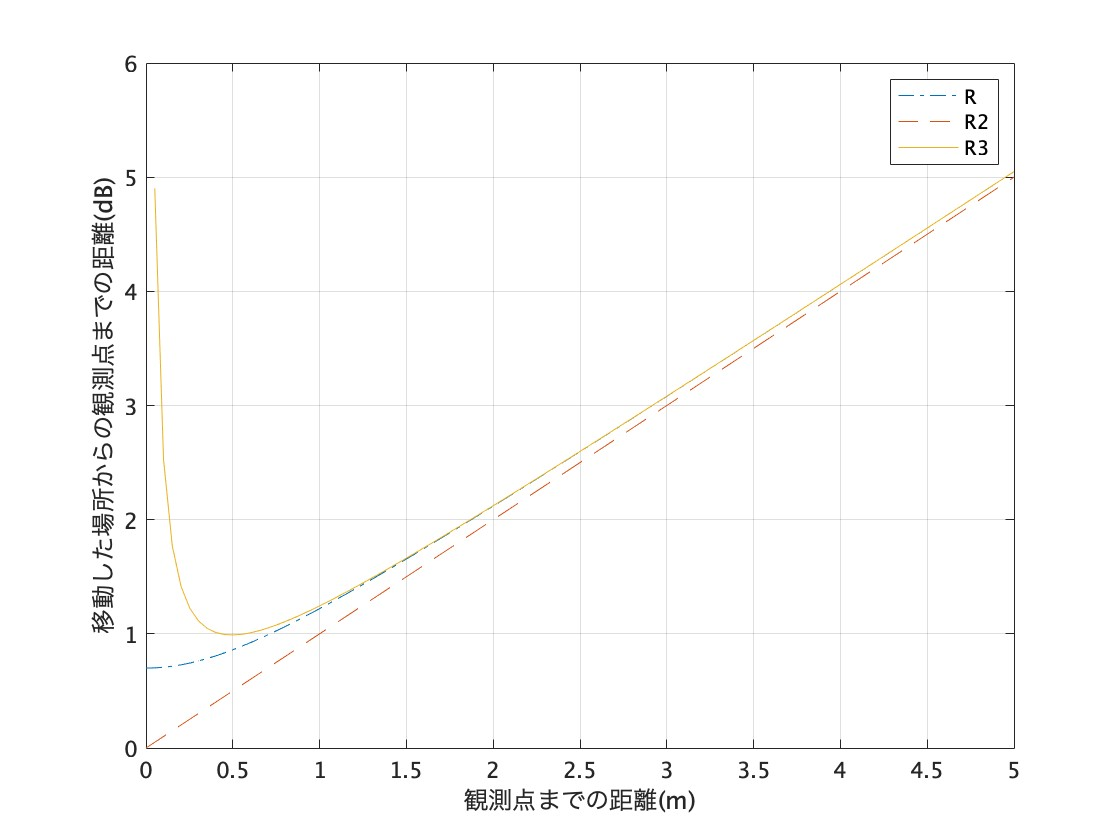
\includegraphics[scale=0.3]{week4_1.jpg}
  \caption{}
\end{figure}

\subsection{D=10波長のとき}
Dは10波長であるので、\begin{math} y'=5\lambda\end{math}とし、\begin{math}
  \lambda = 0.7\end{math}の時のR,R2,R3のグラフは以下のようになる。

\begin{figure}[h]
  \centering
  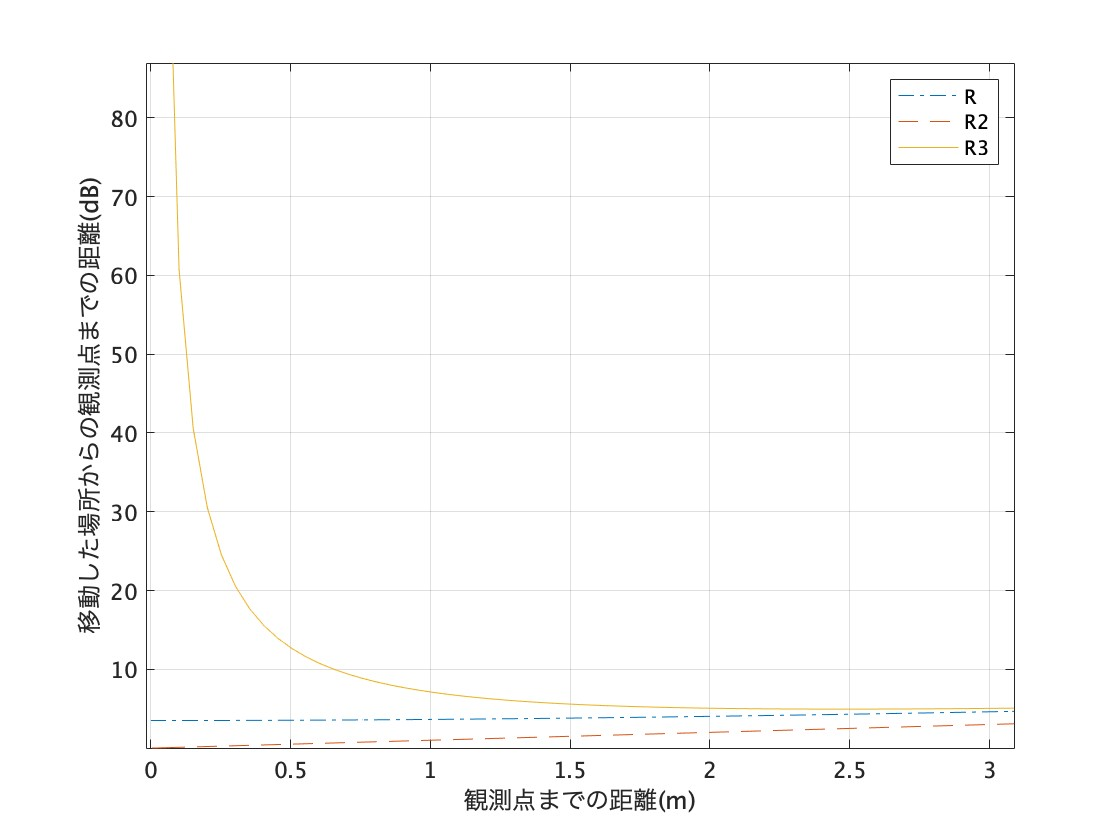
\includegraphics[scale=0.3]{week4_2.jpg}
  \caption{}
\end{figure}

\section{}

観測点がx軸上から60度方向にあるので、\begin{math} \theta = \frac{\pi}{6} \end{math}
となる,よって

\begin{align*}
  R = (r^2 + (-\sqrt{3}ry'+y'^{\,2}))^{\frac{1}{2}}
\end{align*}

\begin{align*}
  R = r - \frac{\sqrt{3}}{2}y' + \frac{y'^{\,2}}{8r} + \frac{\sqrt{3}y'^{\,3}}{16r^2} + \cdots
\end{align*}

となる、よって第二項から第四項までの式を以下のように表す。

\begin{align*}
  R2 &= r - \frac{\sqrt{3}}{2}y'\\
  R3 &= r - \frac{\sqrt{3}}{2}y' + \frac{y'^{\,2}}{8r} \\
  R4 &= r - \frac{\sqrt{3}}{2}y' + \frac{y'^{\,2}}{8r} + \frac{\sqrt{3}y'^{\,3}}{16r^2}
\end{align*}


\subsection{D=2波長のとき}

Dは2波長であるので、\begin{math} y'=\lambda\end{math}とし、\begin{math}
  \lambda = 0.7\end{math}の時のR,R2,R3,R4のグラフは以下のようになる。

\begin{figure}[h]
  \centering
  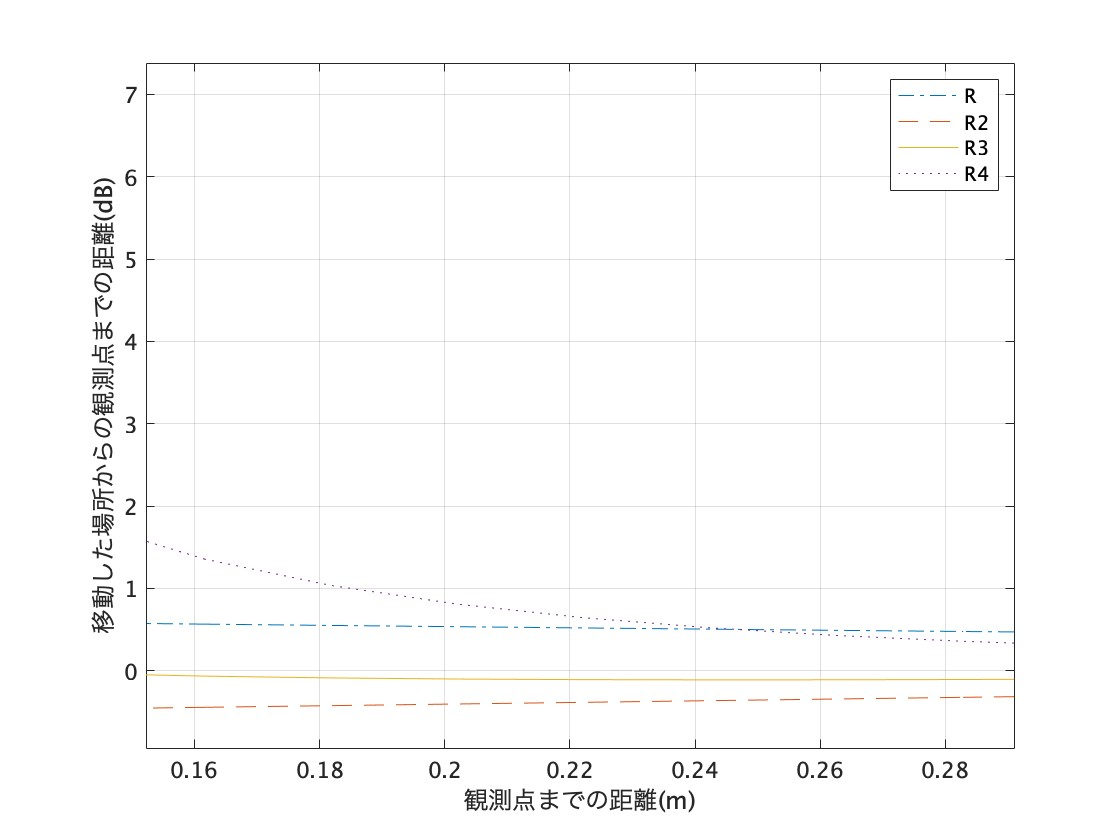
\includegraphics[scale=0.3]{week4_3.jpg}
  \caption{}
\end{figure}


\subsection{D=10波長のとき}

Dは10波長であるので、\begin{math} y'=5\lambda\end{math}とし、\begin{math}
  \lambda = 0.7\end{math}の時のR,R2,R3,R4のグラフは以下のようになる。
\begin{figure}[h]
  \centering
  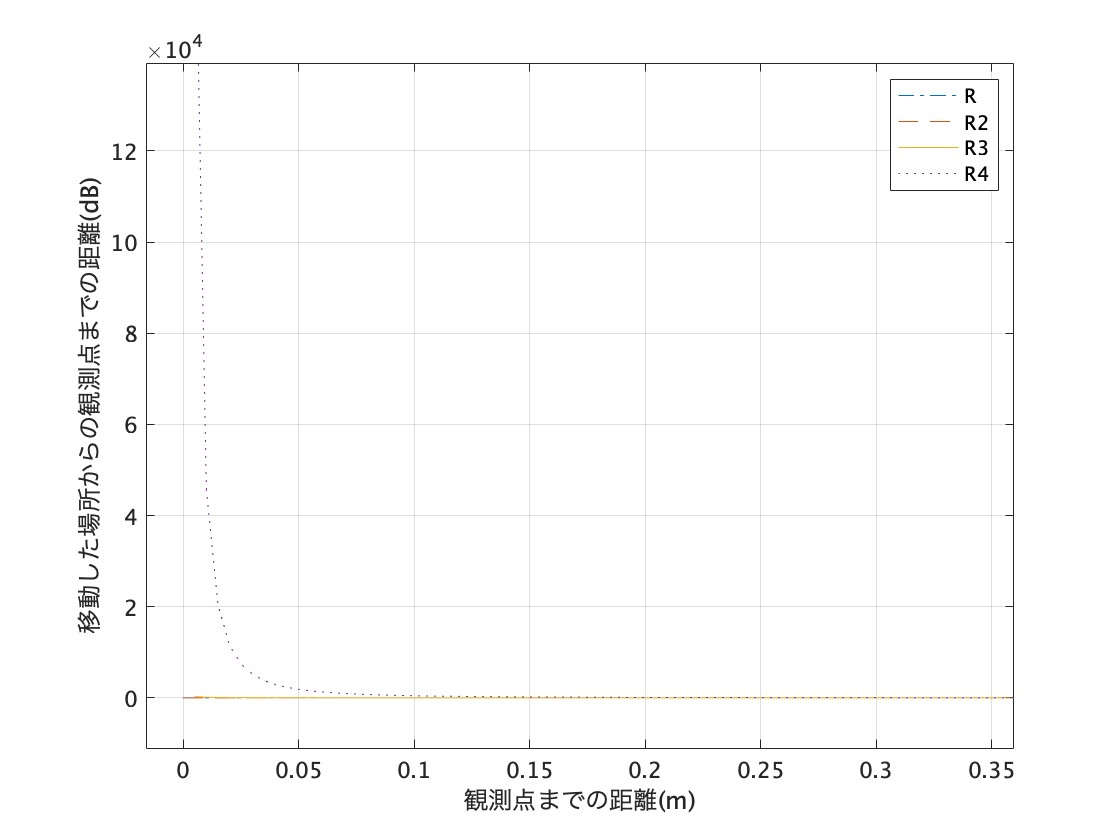
\includegraphics[scale=0.3]{week4_4.jpg}
  \caption{}
\end{figure}



\end{document}

